\begin{center}
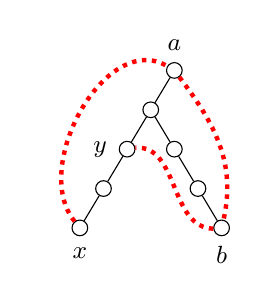
\begin{tikzpicture}[scale=.5,level distance=10mm, state/.style={circle, draw, minimum size=1mm}]]
  \tikzstyle{every node}=[font=\small, draw=black,circle,inner sep=2pt, minimum size=1mm]
  \tikzstyle{level 1}=[sibling distance=12mm, set style={{every node}+=[draw=black]}]
  \tikzstyle{level 2}=[sibling distance=12mm, set style={{every node}+=[draw=black]}]
  \tikzstyle{level 3}=[sibling distance=12mm,  set style={{every node}+=[draw=black]}]
  \tikzstyle{level 4}=[sibling distance=12mm,  set style={{every node}+=[draw=black]}]
  \tikzstyle{level 5}=[sibling distance=12mm,  set style={{every node}+=[draw=black]}]

    \node [label=above:{$a$}] (a) {}
     child {
        node {}
              child {node (y)[label=left:{$y$}] {}
                child {node {} 
                child{node[label=below:{$x$}] (x) {}}
                child[fill=none] {edge from parent[draw=none]}
                }
                child[fill=none] {edge from parent[draw=none]}
                }
                child {node {}
                child[fill=none] {edge from parent[draw=none]}
                child {node {}
                child[fill=none] {edge from parent[draw=none]}
                child {node[label=below:{$b$}] (b) {}}}
                }
            }
    child[fill=none] {edge from parent[draw=none]};
    
    \draw[-,dotted,ultra thick,relative,red] (x) to[out=70,in=90] (a);
    
    \draw[-,dotted,ultra thick,relative,red] (a) to[out=20,in=150] (b);

    \draw[-,dotted,ultra thick,relative,red] (b) to[out=45,in=230] (y);
       
\end{tikzpicture}
\end{center}